\chapter{Applications: Analysis of HPC/GPU programs}
\section{Motivation}
Due to FJ, Cilk, X10, DPJ, TPL, CUDA there's renewed interest in structured parallel languages. Determinism is wanted in applications that use such languages. There are lots of parallel algorithmis: Scientific Computing, Signal Processing, Encryption, Sorting, Searching, String Indexing\\
\textbf{Determinism}: for the same input, produce the same output.

\section{Goal}
Prove determinism. Any pair of terminating executions starting with \underline{equivalent input} states, end in \underline{equivalent output} states. Proving arbitrary programs deterministic is hard, instead, we prove a \underline{stronger} property which implies determinism: \textbf{Conflict-Freedom} meaning, parallel threads always access disjoint memory.
\begin{enumerate}
\item Compute all reachable concrete states
\item Check if each state is conflict-free
\end{enumerate}
We denote conflict as a state where 2 threads are \underline{enabled} to access the \underline{same} memory location and one of these accesses is a write.
\textbf{Checking Conflict-Freedom is potentially unbounded.}

\section{Conflict-free Checker}
\label{conflict_free_checker}
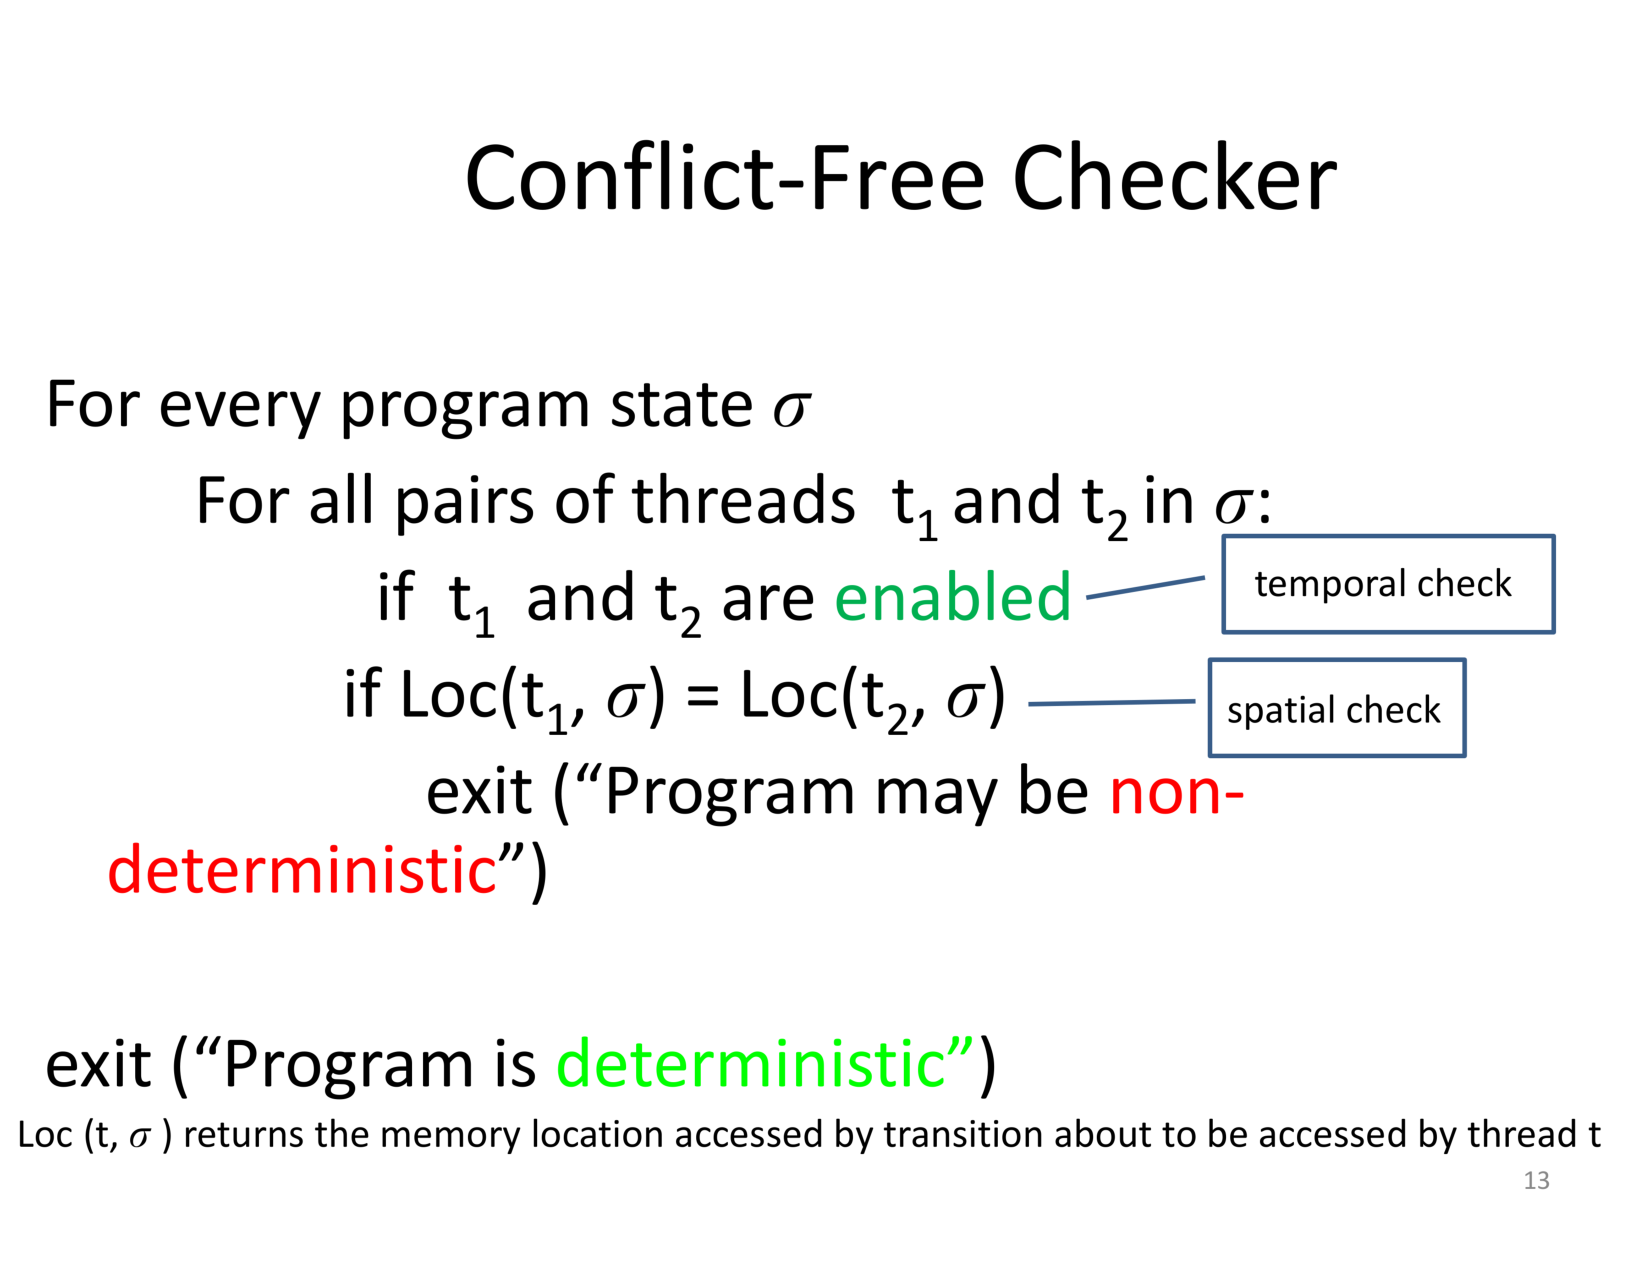
\includepdf[pages={-}]{pages/conflict_free_checker.pdf}

\section{Unboundedness}
Heap, range of array indices and number of threads is unbounded. \\
\textbf{Dealing with Unboundedness}
\begin{itemize}
\item Unbounded Heap
\begin{itemize}
\item Compute finite set of abstract locations
\item Using flow-insensitive \textbf{points-to analysis}
\end{itemize}
\item Unbounded range of array indices
\begin{itemize}
\item Compute symbolic index constraints
\item Using \textbf{numerical abstractions}
\end{itemize}
\item Unbounded number of threads (not discussed in class)
\end{itemize}
\subsection{Points-to Analysis}
\subsubsection{Terms}
Two pointers p and q are \underline{aliases} if they point to the same memory location. $(p,A)$ is a \underline{points-to pair} where $p$ holds the address of object $A$. For two points-to pairs $(p,A),(r,A)$ $p$ and $r$ are aliases.
\subsubsection{Allocation Sites}
Heap is divided into a fixed partitions. All objects \underline{allocated at the same program point} ge represented by a single "abstract object".
\section{Flow-Insensitive Analysis}
Just ignore if conditions and look at every statement for points-to analysis. E.g
\begin{verbatim}
p := new Array 5; // allocation site A1
q := new Array 5; // allocation site A2
if p=q then
	z := p
else
	z := q
\end{verbatim}
will output $points-to(z)={A1, A2}$.

\section{Computing abstract states}
Using \underline{sequential} analysis (based on numerical analysis and pointer analysis) we compute for each thread. \textbf{see Page 34}. First we build for each label (program line) the \underline{abstract states}. E.g. $\sigma_1=\{pc=1,idx=2*tid-ps\}$ for a first program line looking like: \begin{verbatim}
void update(double[][] G, int start, int last, double c1, double c2, int nm, int ps){
   for(tid=start; tid<last; tid+=1){
1:     double [] Gi = G[i];
...
   }
}
\end{verbatim}
For each thread id ($tid$) we can the build \underline{cartesian states}. E.g for $tid=1$ and label 1 ($pc_1=1$):\\
$pc_1=1,ps=0,idx_1=2\\
pc_1=1,ps=1,idx_1=1\\
pc_1=1,ps=2,idx_1=0$\\
And for $tid=4$:\\
$pc_4=1,ps=0,idx_4=8\\
pc_4=1,ps=3,idx_4=5\\
pc_4=1,ps=7,idx_4=1$\\
Combining cartesian states for different threads will give us the \underline{program states}: \\
$pc_1=1,idx_1=2,pc_4=1,idx_4=8,ps=0$ \\
Since $ps$ is a parameter to the function combining two cartesian states with different $ps$ values does not make sense. But it's OK to combine two threads but on different program lines ($pc_i=k,pc_j=k',k\neq k',i\neq j$).\\
\textbf{Summary}:
\begin{itemize}
\item compute invariants for each thread. denote computed values using an expression
\item build cartesian states. "fill" in the missing values to compute variables (many possible combinations).
\item combine abstract states for different threads.
\end{itemize}
Recall the conflict free checker: \ref{conflict_free_checker}. Using the abstract states we can now define an abstract conflict-free checker:
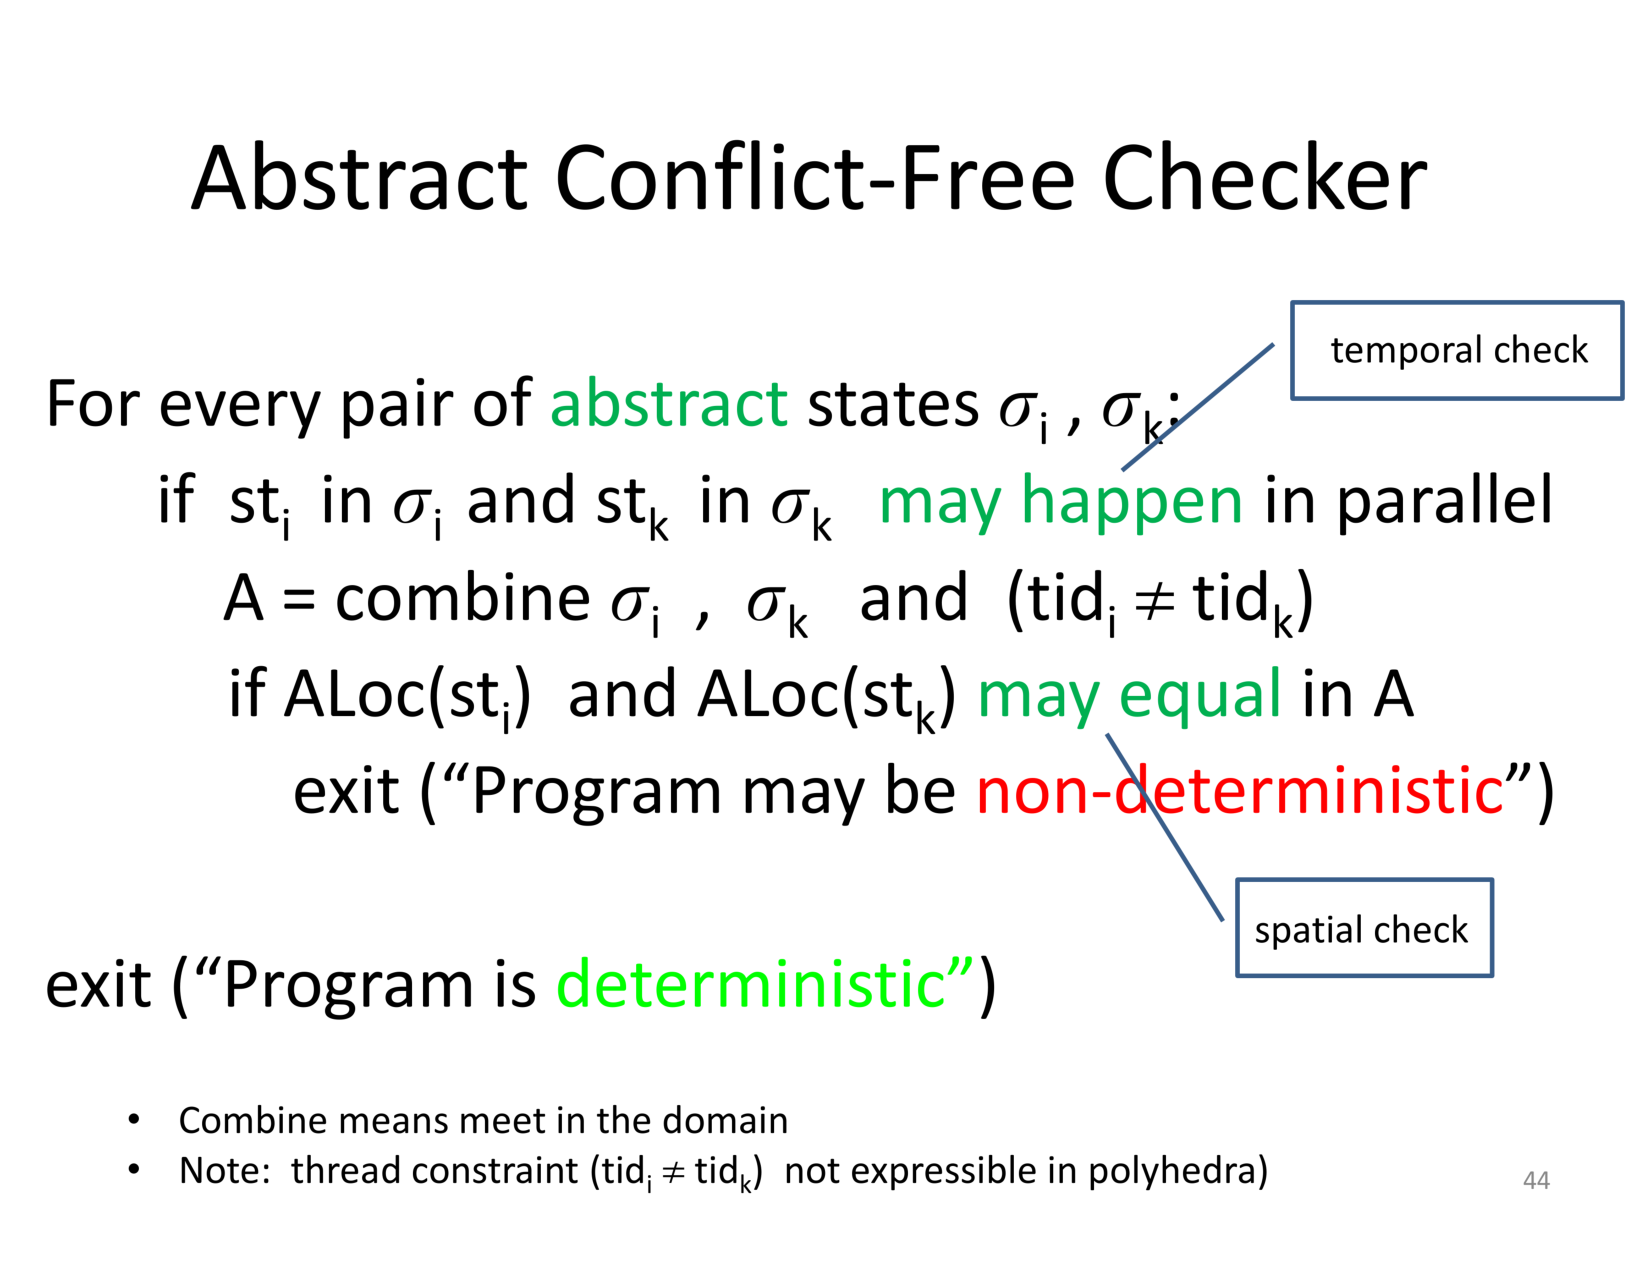
\includepdf[pages={-}]{pages/abstract_conflict_free_checker.pdf}
A \underline{may happen} analysis can be used for the may happen parts. There are many works on this. \textbf{TODO}?
\section{May Equal (Arrays) / Abstract Locations}
$ALoc(G[i]=128) := (G,i)$ with $G$ a pointer- and $i$ and integer variable. When may two $ALoc(a,i)$ and $ALoc(b,k)$ equal? When $(a $ may alias $ b) \wedge (i $ may overlap $ k)$. With may alias=$points-to(a) \cap points-to(b) \neq \emptyset$ and may overlap=$A_N \sqcap (i=k)\neq \bot$ \textbf{TODO: not sure what $A_n$ is. page 49}
\section{Caveats}
Heap abstraction is imprecise. 
\begin{itemize}
\item Aliasing information \underline{inside} reference arrays is lost. Example: \begin{verbatim}
Object A[], double G[][];
\end{verbatim}
\item So, points-to information is not enough
\item We want $\forall i,j,A:i \neq j \implies A[i] \neq A[j]$ but this is very difficult to prove in general.
\end{itemize}
\subsection{Domain-specific solution}
Most numerical HPC/GPU programs initialize reference arrays only with fresh objects \textit{A[i] = new Object();} and never update afterwards. Easy to prove as a global invariant.
\section{Implementation}
\begin{itemize}
\item Soot (Analysis works on Jimple intermediate representation)
\item Apron library (for numerical invariants)
\item Benchmarked using Java JGF benchmarks
\end{itemize}

\section{Limitations}
\begin{itemize}
\item cannot handle some kinds of non-linear constraints (\textit{A[x*N + z]=c} where N never changes
\item atomic sections
\item Accesses from nested primitive arrays: \textit{A[ B[i] ] = 5} where \textit{B[i]}'s are distinct
\end{itemize}
\section{Recap}
To automatically prove determinism prove a \underline{stronger property}: conflict-freedom.